\renewcommand{\theequation}{\theenumi}
\renewcommand{\thefigure}{\theenumi}
\renewcommand{\thetable}{\theenumi}
\begin{enumerate}[label=\thesection.\arabic*.,ref=\thesection.\theenumi]
\numberwithin{equation}{enumi}
\numberwithin{figure}{enumi}
\numberwithin{table}{enumi}
%
\item 
Let $X_{1},X_{2},\dots$ be independent and identically distributed random variables each following a uniform distribution on (0,1). Denote 
\begin{align}
T_{n}=\max\cbrak{ X_{1},X_{2},\dots,X_{n}}. 
\end{align}
Then, which of the following statements are true?
\begin{enumerate}
    \item $T_{n}$ converges to 1 in probability.
    \item $n(1-T_{n})$ converges in distribution.
    \item $n^{2}(1-T_{n})$ converges in distribution.
    \item $\sqrt{n}(1-T_{n})$ converges to 0 in probability.
\end{enumerate}
%
\solution
\begin{definition}
{\em Random Sampling :}
A collection of random variables $X_{1},X_{2},\dots,X_{n}$ is said to be a random sample of size $n$ if they are independent and identically distributed, i.e,
\begin{enumerate}
    \item $X_{1},X_{2},\dots,X_{n}$ are independent random variables
    \item They have the same distribution (Let us denote it by $F_{X}(x)$), i.e,
    \begin{align}
        F_{X}(x)=F_{X_{i}}(x), i = 1,2,\dots,n \forall x\in \mathbb{R}
    \end{align}
\end{enumerate}
\end{definition}
\begin{definition}
{\em Order Statistics :}
Given a random sample $X_{1},X_{2},\dots,X_{n}$, the sequence $X_{(1)},X_{(2)},\dots,X_{(n)}$ is called the order statistics of it. Here,
\begin{align}
    &X_{(1)}=\min\brak{X_{1},X_{2},\dots,X_{n}}\\
    &X_{(2)}=\text{the }2^{nd}\text{ smallest of }X_{1},X_{2},\dots,X_{n}\\
    &\vdots\\
    &X_{(n)}=\max\brak{X_{1},X_{2},\dots,X_{n}}
\end{align}
\end{definition}
\begin{lemma}
{\em Distribution of the maximum :}
\begin{align}
	\label{eq:conv/1/pdf}
    f_{T_{n}}(x)&=\begin{cases}
	nx^{n-1}, & 0< x<1 \\~\\[-1em]
	0, & otherwise
	\end{cases}\\
	F_{T_{n}}(x)&=\begin{cases}
	x^{n}, & 0< x<1 \\~\\[-1em]
	1, & x\geq 1\\~\\[-1em]
	0, & otherwise
	\end{cases} 
	\label{eq:conv/1/cdf}
\end{align}
\end{lemma}
%\proof
Proof:
\begin{align}
   F_{X_{(n)}}(x)&=\pr{X_{(n)}\leq x}\\
   &=\pr{X_{1}\leq x,X_{2}\leq x,\dots,X_{n}\leq x}\\
   &=\pr{X_{1}\leq x}\pr{X_{2}\leq x}\dots\pr{X_{n}\leq x}\\
   \label{conv/1/eq:F}
   &=\sbrak{\pr{X_{1}\leq x}}^{n}\brak{ \text{i.i.d}}\\
   &=\sbrak{F_{X}(x)}^{n}
   \label{eq:conv/1/cdf/max}
\end{align}
and 
\begin{align}
   f_{X_{(n)}}(x)&=\dfrac{d}{dx}\brak{F_{X_{(n)}}(x)}=\dfrac{d}{dx}\brak{\sbrak{F_{X}(x)}^{n}}\\
   &=n\brak{\sbrak{F_{X}(x)}^{n-1}}\dfrac{d}{dx}\brak{F_{X}(x)}\\
%   \label{conv/1/eq:f}
   &=n\sbrak{F_{X}(x)}^{n-1}f_{X}(x)
   \label{eq:conv/1/pdf/max}
\end{align}
$\because $
\begin{align}
    f_{X_{i}}(x)&=\begin{cases}
	1, & 0< x<1 \\~\\[-1em]
	0, & otherwise
	\end{cases},
	\\
	F_{X_{i}}(x)&=\begin{cases}
	x, & 0< x<1 \\~\\[-1em]
	1, & x\geq 1\\~\\[-1em]
	0, & otherwise,
	\end{cases} 
\end{align}
$\forall i\in \mathbb{N}$.  Substituting the above in    \eqref{eq:conv/1/pdf/max} and \eqref{eq:conv/1/cdf/max} yields 	\eqref{eq:conv/1/pdf} and 	\eqref{eq:conv/1/cdf} respectively. 
Then, as $T_{n}=max\{ X_{1},X_{2},\dots,X_{n}\}=X_{(n)}$,
\begin{lemma}
If $Y=aX+b$ and $a<0$, then
\begin{align}
\label{conv/1/eq:form}
    F_{Y}(y)=1-F_{X}\brak{\dfrac{y-b}{a}}
\end{align}
\end{lemma}
\begin{definition}
{\em	Convergence in Probability :}
A sequence of random variables $X_{1},X_{2},X_{3},\dots$ converges in probability to a random variable $X$, shown by $X_{n}\xrightarrow[]{p}X$, if
\begin{align}
    \displaystyle\lim_{n\to\infty}\pr{|X_{n}-X|\geq\epsilon}=0,\forall\epsilon>0
\end{align}
\end{definition}
%
\begin{definition}
	{\em Convergence in Distribution :}
A sequence of random variables $X_{1},X_{2},X_{3},\dots$ converges in distribution to a random variable $X$, shown by $X_{n}\xrightarrow[]{d}X$, if
\begin{align}
    \displaystyle\lim_{n\to\infty}F_{X_{n}}(x)=F_{X}(x)
\end{align}
for all $x$ at which $F_{X}(x)$ is continuous.
\end{definition}
%
\begin{enumerate}
\item 
%To evaluate : $\displaystyle\lim_{n\to\infty}\pr{|T_{n}-1|\geq\epsilon},\forall\epsilon>0$
\begin{multline}
    \displaystyle\lim_{n\to\infty}\pr{|T_{n}-1|\geq\epsilon}=\displaystyle\lim_{n\to\infty}\pr{1-T_{n}\geq\epsilon}\\
	=\displaystyle\lim_{n\to\infty}\pr{T_{n}\leq1-\epsilon}=\displaystyle\lim_{n\to\infty}F_{T_{n}}(1-\epsilon)
	\label{conv/1/1/cdf}
\end{multline}
\begin{align}
    \because F_{T_{n}}(1-\epsilon)=\begin{cases}
	(1-\epsilon)^{n}, & 0< \epsilon<1 \\~\\[-1em]
	0, & \epsilon\geq 1
	\end{cases}
	\label{conv/1/1/cdf/epsilon}
\end{align}
and 
\begin{align}
	\label{conv/1/1/cdf/epsilon/lim}
    \because\displaystyle\lim_{n\to\infty}(1-\epsilon)^{n}=0 \text{ for } 0< \epsilon<1\\
\end{align}
%
from 	\eqref{conv/1/1/cdf/epsilon/lim}, 	\eqref{conv/1/1/cdf/epsilon} and 	\eqref{conv/1/1/cdf},
\begin{align}
	 \displaystyle\lim_{n\to\infty}\pr{|T_{n}-1|\geq\epsilon}=0,\forall\epsilon>0
\end{align}
$\therefore T_{n}$ converges to 1 in probability.
\item 
Substituting $a=-n,b=n$ in \eqref{conv/1/eq:form},
\begin{align}
	F_{n(1-T_{n})}(x)=1-F_{T_{n}}\brak{1-\dfrac{x}{n}}\\
\end{align}	
where
\begin{align}
    F_{T_{n}}\brak{1-\dfrac{x}{n}}=\begin{cases}
	\brak{1-\dfrac{x}{n}}^{n}, & 0< x<n \\~\\[-1em]
	1, & x\leq 0\\~\\[-1em]
	0, & x\geq n
	\end{cases} \\
	from  	\eqref{eq:conv/1/cdf}
\end{align}
\begin{align}
	\because\displaystyle\lim_{n\to\infty}\brak{1-\dfrac{y}{n}}^{n}=e^{-y}, \\
\end{align}
\begin{align}
\therefore\displaystyle\lim_{n\to\infty} F_{T_{n}}\brak{1-\dfrac{x}{n}}&=\begin{cases}
	e^{-x}, & x>0 \\~\\[-1em]
	1, & x\leq 0
	\end{cases} \\
	\implies 
	\displaystyle\lim_{n\to\infty}F_{n(1-T_{n})}(x)&=1-\displaystyle\lim_{n\to\infty} F_{T_{n}}\brak{1-\dfrac{x}{n}}
\end{align}
which can be expressed as
\begin{align}
\label{conv/1/eq:cdf1}
    \therefore\displaystyle\lim_{n\to\infty} F_{n(1-T_{n})}(x)=\begin{cases}
	1-e^{-x}, & x>0 \\~\\[-1em]
	0, & x\leq 0
	\end{cases} 
\end{align}
$\therefore n(1-T_{n})$ converges in distribution to the random variable $X\sim Exponential(1)$.
% \begin{figure}[h!]
% \centering
% \includegraphics[width=\linewidth]{Assignment9}
% \caption{CDF}
% \label{conv/1/plot}
% \end{figure}
\item 
Substituting $a=-n^{2},b=n^{2}$ in \eqref{conv/1/eq:form},
\begin{align}
    F_{n^{2}(1-T_{n})}(x)&=1-F_{T_{n}}\brak{1-\dfrac{x}{n^{2}}}\\
    F_{T_{n}}\brak{1-\dfrac{x}{n^{2}}}&=\begin{cases}
	\brak{1-\dfrac{x}{n^{2}}}^{n}, & 0< x<n^{2} \\~\\[-1em]
	1, & x\leq 0\\~\\[-1em]
	0, & x\geq n^{2}
	\end{cases} \\
	&=\begin{cases}
		1, & x>0 \\~\\[-1em]
		1, & x\leq 0
		\end{cases} 
	\end{align}
	\begin{align}
	\because\displaystyle\lim_{n\to\infty}\brak{1-\dfrac{x}{n^{2}}}^{n}=1
%&\therefore\displaystyle\lim_{n\to\infty} F_{T_{n}}\brak{1-\dfrac{x}{n^{2}}}
	\end{align}
	yielding 
	\begin{align}
%&\because\displaystyle\lim_{n\to\infty}F_{n^{2}(1-T_{n})}(x)=1-\displaystyle\lim_{n\to\infty} F_{T_{n}}\brak{1-\dfrac{x}{n^{2}}}\\
\label{conv/1/eq:cdf2}
    \displaystyle\lim_{n\to\infty} F_{n^{2}(1-T_{n})}(x)=\begin{cases}
	0, & x>0 \\~\\[-1em]
	0, & x\leq 0
	\end{cases} 
\end{align}
which is not a valid CDF.  Hence, 
%$\because$ The CDF in \eqref{conv/1/eq:cdf2} is not valid,\\
$ n^{2}(1-T_{n})$ does not converge in distribution.
\item 
% Convergence in Probability :\\
% A sequence of random variables $X_{1},X_{2},X_{3},\dots$ converges in probability to a random variable $X$, shown by $X_{n}\xrightarrow[]{p}X$, if
% \begin{align}
%     \displaystyle\lim_{n\to\infty}\pr{|X_{n}-X|\geq\epsilon}=0,\forall\epsilon>0
% \end{align}
% To evaluate :\\ $\displaystyle\lim_{n\to\infty}\pr{|\sqrt{n}(1-T_{n})-0|\geq\epsilon},\forall\epsilon>0$
\begin{multline}
	\displaystyle\lim_{n\to\infty}\pr{|\sqrt{n}(1-T_{n})-0|\geq\epsilon}    \\ =\displaystyle\lim_{n\to\infty}\pr{1-T_{n}\geq\dfrac{\epsilon}{\sqrt{n}}}\\
    =\displaystyle\lim_{n\to\infty}\pr{T_{n}\leq1-\dfrac{\epsilon}{\sqrt{n}}}\\
	=\displaystyle\lim_{n\to\infty}F_{T_{n}}\brak{ 1-\dfrac{\epsilon}{\sqrt{n}}}
	\\
	=\begin{cases}
		\brak{1-\dfrac{\epsilon}{\sqrt{n}}}^{n}, & 0< \epsilon< \sqrt{n}\\~\\[-1em]
		0, & \epsilon\geq \sqrt{n}
		\end{cases}
\end{multline}
\begin{multline}
%    &F_{T_{n}}\brak{1-\dfrac{\epsilon}{\sqrt{n}}}\\
    \because\displaystyle\lim_{n\to\infty}\brak{1-\dfrac{\epsilon}{\sqrt{n}}}^{n}=0 \text{ for } 0< \epsilon<\sqrt{n},\\
     \displaystyle\lim_{n\to\infty}\pr{|\sqrt{n}(1-T_{n})-0|\geq\epsilon}=0,\forall\epsilon>0
\end{multline}
$\therefore\sqrt{n}(1-T_{n})$ converges to 0 in probability.
\end{enumerate}
\begin{lstlisting}
Hence, options 1), 2), 4) are correct.
\end{lstlisting}
%
\item Let $\{X_i\}_{i \geq 1}$ be a sequence of i.i.d. random variables with $\mean{X_i}=0$ and $\var{X_i}=1$. Which of the following are true?
%
\begin{enumerate}
    \setlength{\itemsep}{2pt}
    \item $\dfrac{1}{n} \sum_{i=1}^n X_i^2 \to 0$ in probability 
    \item $\dfrac{1}{n^{3/4}} \sum_{i=1}^n X_i \to 0$ in probability 
    \item $\dfrac{1}{n^{1/2}} \sum_{i=1}^n X_i \to 0$ in probability 
    \item $\dfrac{1}{n} \sum_{i=1}^n X_i^2 \to 1$ in probability
\end{enumerate}
%
\solution
\begin{definition}
    (Convergence in distribution)\\
    A sequence of random variables $Y$, $Y_1$, $Y_2 \ldots$   converges in distribution to a random variable $Y$, if
    \begin{align}
        \lim_{n \to \infty}F_{X_{n}} (a) = F_{X} (a)  \text{  }\forall a \in \mathbb{R}.
    \end{align}
\end{definition}
\begin{definition} \label{conv/2/def2}
    (Convergence in probability)\\
    A sequence of random variables $Y$, $Y_1$, $Y_2 \ldots$ is said to converge in probability to $Y$, if
    \begin{align}
        \lim_{n \to \infty}\pr{\abs{Y_n - Y} > \epsilon} = 0  \text{  }\forall \epsilon > 0.
    \end{align}
\end{definition}
\begin{lemma}\label{conv/2/lma1}
    If
    \begin{math}
    {Y_n} \to Y \text{ in probability, }{Y_n} \to Y \text{ in distribution.}
    \end{math}
\end{lemma}
\begin{lemma}\label{conv/2/lma3}
    (Strong Law of Large Numbers)\\ 
Let $X_1$, $X_2$, \ldots $X_n$ be i.i.d. random variables with expected value $E(X_i)=\mu < \infty$, then,
\begin{align}
%    \lim_{n \to \infty}\pr{\left|\dfrac{1}{n}\sum_{i=1}^n X_i - \mu \right|\geq \epsilon}=0
X_i \xrightarrow[]{p}\mu
\end{align}
Or, 
\begin{align}
    \dfrac{1}{n}\sum_{i=1}^n X_i \xrightarrow[]{p} \mu
\end{align}
%
\end{lemma}
\begin{lemma} \label{conv/2/lmaconda}
    If $X_i$ is a sequence of i.i.d. random variables, with
    \begin{align}
        \label{conv/2/maincondA}
        F_{X_i}(x)=F_X(x),
    \end{align}
    then,
    \begin{align}
        F_{X_i^2}(x)=F_{X^2}(x)
    \end{align}
    $\forall x \in \mathbb{R}$, where $F_{X}(x)$ is the c.d.f. of $X_i$.
\end{lemma}
\begin{proof}
% ${X_i}$ is a sequence of i.i.d. random variables, which means it satisfies the following condition.
% \begin{align}
%         F_{X_1}(x)=F_{X_2}(x)&=\ldots=F_{X_n}(x)=F_X(x) 
% \end{align}
% where $F_X(x)$ is the c.d.f. of $X_i$.
% Let $Y_i=X_i^2$. For $y \geq 0$,
\begin{align}
    F_{{X_i}^2}(y) &=\pr{X_i^2 \leq y}
%     &=\pr{Y_i \leq y}\\
%     \implies F_{Y_i}(y)
% \end{align}
% \begin{align}
    \\
    \implies F_{Y_i}(y)&=\pr{-\sqrt{y} \leq X_i \leq \sqrt{y}}\label{conv/2/eqref}\\
%     \implies F_{Y_i}(y)&=\pr{X_i \leq \sqrt{y}}-\pr{X_i \leq -\sqrt{y}}
% \end{align}
% \begin{align}
\implies   F_{{X_i}^2}(y)&=F_{X_i}(\sqrt{y})-F_{X_i}(-\sqrt{y})
\\
&= F_{X}(\sqrt{y})-F_{X}(-\sqrt{y}) 
\\
&= F_{{X}^2}(y)
\end{align}
Using \eqref{conv/2/maincondA},
% \begin{align} 
%     F_{Y_i}(y)&=F_X(\sqrt{y})-F_X(-\sqrt{y})\label{conv/2/eqY}
% \end{align}
% From \eqref{conv/2/eqY},
% \begin{align} 
%     F_{Y_1}(y)=F_{Y_2}(y)=\ldots=F_{Y_n}(y)=F_Y(y)\label{conv/2/condnA}
% \end{align}
% where $F_Y(y)$ is the c.d.f. of $Y_i=X_i^2$.
\end{proof}
\begin{corollary} \label{conv/2/xi2lma}
    If $X_i$ are i.i.d, $X_i^2$ are i.i.d.
    % \begin{align}
    %     F_{X_1,\ldots X_n}(x_1\ldots x_n)&=F_X(x_1)F_X(x_2)\ldots F_X(x_n)\label{conv/2/maincondnB}
    % \end{align} 
    % where $F_{X}(x)$ is the c.d.f. of $X_i$, then for $Y_i = X_i^2$
    % \begin{align}
    % F_{Y_1,Y_2,\dots,Y_n}&(y_1,y_2,\dots,y_n)=F_Y(y_1)F_Y(y_1)\dots F_Y(y_n)
    % \end{align}
%    where $F_Y(y)$ is the c.d.f. of 
\end{corollary}
\begin{proof}
Let $Y_i = X_i^2$.
%Now, for $y_i\geq0$, consider
\begin{multline}
    F_{Y_1,Y_2,\ldots,Y_n}(y_1,y_2,\ldots,y_n)
\\=\pr{Y_1 \leq y_1,Y_2 \leq y_2,\ldots,Y_n \leq y_n}
     \\=\pr{X_1^2 \leq y_1,X_2^2 \leq y_2,\ldots,X_n^2 \leq y_n}
    %\\=\pr{-\sqrt{y_1} \leq X_1 \leq \sqrt{y_1},\ldots,-\sqrt{y_n} \leq X_n \leq \sqrt{y_n}}
    \\ = \prod_{i=1}^{n}\sbrak{\pr{-\sqrt{y_i} \leq X_i \leq \sqrt{y_i}}}
    \\= \prod_{i=1}^{n}F_Y(y_i) 
 \end{multline}
$\implies X_i^2$ are i.i.d.
% So,
% \begin{align} \label{conv/2/condnB}
%     F_{Y_1,Y_2,\dots,Y_n}&(y_1,y_2,\dots,y_n)\nonumber \\
%     &=F_Y(y_1)F_Y(y_1)\dots F_Y(y_n)
% \end{align}
\end{proof}
% \begin{lemma} 
% If ${X_i}$ is a sequence of i.i.d. random variables, it follows that $X_i^2$ is also a sequence of i.i.d. random variables.
% \end{lemma}
% \begin{proof}
%     From Lemma \ref{conv/2/lmaconda} and Lemma \ref{conv/2/lmacondb}, $X_i^2$ is also a sequence of i.i.d. random variables.
% \end{proof}
\begin{lemma} \label{conv/2/varsum}
    If $X_1, X_2, \ldots X_n$ are independent random variables,
    \begin{align}
        \var{\sum_{i=1}^n X_i} = \sum_{i=1}^{n}\var{X_i}
    \end{align}
\end{lemma}
\begin{lemma}\label{conv/2/lma4}
    (Chebyshev's Inequality)\\
Let the random variable $X$ have a finite mean $\mu$ and a finite variance $\sigma^2$. For every $\epsilon>0$, 
\begin{align}
    \pr{\abs{X - \mu} \geq \epsilon} \leq \frac{\sigma^2}{\epsilon^2}
\end{align}
\end{lemma}
\begin{lemma}\label{conv/2/lma2}
    (Central Limit Theorem)
Let $X_1$, $X_2$, \ldots $X_n$ be i.i.d. random variables with expected value $E(X_i)=\mu < \infty$  and $0 < V(X_i)=\sigma^2 < \infty$. Then the random variable 
\begin{align}
    Z_n 
%    = \frac{\bar{x} - \mu}{\frac{\sigma}{\sqrt{n}}} 
    = \frac{\sum_{i=1}^n X_i - n\mu}{\sqrt{n}\sigma}
    \xrightarrow[]{d} \gauss{0}{1}
\end{align}
% converges in distribution to the standard normal random variable as n goes to infinity, that is
% \begin{align}
%     \lim_{n \to \infty}\pr{Z_n \leq a} = \Phi(a)   \text{        }\forall a \in \mathbb{R}.
% \end{align}
% where $\Phi(a)$ is the standard normal CDF.
\end{lemma}
\begin{enumerate}
\item 
From Lemma \ref{conv/2/xi2lma}, \{$X_i^2$\} is a sequence of i.i.d. random variables.  Hence, 
%Now, we know,
\begin{align}
    E(X_i^2)=\var{X_i}+\sbrak{\mean{X_i}}^2 = 1
\end{align}
% Putting given values, we get,
% \begin{align} 
%     E(X_i^2)&=1 \label{conv/2/muval}
% \end{align}
From Lemma \ref{conv/2/lma3},  
\begin{align} \label{conv/2/opt4}
   \dfrac{1}{n}\sum_{i=1}^n X_i^2 \xrightarrow[]{p} 1 \ne 0 
\end{align}
Therefore, option 1 is incorrect.
\item 
\begin{lemma} \label{conv/2/result2}
    Let    
    \begin{align}
        Y_n=\dfrac{1}{n^{3/4}}\sum_{i=1}^n X_i,
    \end{align}
    where $X_i$ are i.i.d.  with 
    \begin{align}
        \mean{X_i} = 0, \var{X_i} = 1
            \end{align}
        Then 
        \begin{align}
            \mean{Y_n} = 0,  \var{Y_n} = \dfrac{1}{n^{1/2}} 
                \end{align}
            
\end{lemma}

\begin{proof}
\begin{align}
    \mean{Y_n} &= \dfrac{1}{n^{3/4}}\mean{\brak{\sum_{i=1}^n X_i}} = 0
\end{align}
Since $E(X_i) = 0$. Also, from Lemma \ref{conv/2/varsum},
\begin{align}
    \var{Y_n} &= \dfrac{1}{n^{3/2}} \brak{\sum_{i=1}^n\mean{ X_i}}
    \\
    &= \dfrac{1}{n^{3/2}} \times n = \dfrac{1}{n^{1/2}}
\end{align}
  $\because \var{X_i}=1$. 
\end{proof}
Now, from Lemma \ref{conv/2/lma4} and Lemma \ref{conv/2/result2}
\begin{align}
    \lim_{n \to \infty}\pr{|Y_n-0|\geq \epsilon} &\leq \lim_{n \to \infty }\dfrac{1}{n^{1/2}\epsilon^2}\\
    &= 0
%    \implies &\lim_{n \to \infty}\pr{\left | \dfrac{1}{n^{3/4}}\sum_{i=1}^n X_i - 0 \right|\geq \epsilon}=0
\end{align}
From Definition \ref{conv/2/def2},
\begin{align}
    \dfrac{1}{n^{3/4}}\sum_{i=1}^n X_i \xrightarrow[]{p} 0
\end{align}
Thus, option 2 is correct.
\item Substituting $\mu=0$ and $\sigma=1$, in  Lemma \ref{conv/2/lma2},
\begin{align}
    Z_n &= \dfrac{1}{n^{1/2}} \sum_{i=1}^n X_i  \xrightarrow[]{d} \gauss{0}{1} \ne 0
\end{align}
% From Lemma \ref{conv/2/lma2} 
% \begin{align}
%     \dfrac{1}{n^{1/2}} \sum_{i=1}^n X_i \to  N(0,1)
% \end{align}
% whereas the option states that
% \begin{align}
%  \dfrac{1}{n^{1/2}} \sum_{i=1}^n X_i \to 0
% \end{align} 
% from Lemma \ref{conv/2/lma1}.
Therefore, option 3 is incorrect.
\item From \eqref{conv/2/opt4}, option 4 is correct.
\end{enumerate}
Therefore, options 2 and 4 are correct.
%
\item Let $\{X_{n}\}$ be a sequence of independent random variables where the distribution of $X_{n}$ is normal with mean $\mu$ and variance $n$ for $n$ = 1,2,\dots Define
\begin{align}
    \Bar{X_{n}}&=\frac{1}{n}\sum_{i=1}^{n}X_{i}\\ S_{n}&=\frac{\sum_{i=1}^{n}\frac{1}{i}X_{i}}{\sum_{i=1}^{n}\frac{1}{i}}
\end{align}
Which of the following are true?
\begin{enumerate}
    \item E($\Bar{X_{n}}$) = E($S_{n}$) for sufficiently large $n$
    \label{conv/3/option 1}
    \item Var($S_{n}$) $<$ Var($\Bar{X_{n}}$) for sufficiently large $n$
    \label{conv/3/option 2}
    \item $\Bar{X_{n}}$ is consistent for $\mu$
    \label{conv/3/option 3}
    \item $\Bar{X_{n}}$ is sufficient for $\mu$
    \label{conv/3/option 4}
\end{enumerate}
%
\solution
As $X_{i}$ for $i = 1,2,\dots,n$ are independent random variables we can use this property to state
   \begin{align}
    Var\brak{\sum_{i=1}^{n}g(X_{i})}=\sum_{i=1}^{n}Var(g(X_{i}))\label{conv/3/basic}
    \end{align}
    \begin{definition}\label{conv/3/definition_of_Random_sample}
     Random Sample: The random variables $X_{1},X_{2},X_{3},\dots,X_{n}$ are said to be random sample if
   \begin{enumerate}
       \item the $X_{i}$'s are independent \label{conv/3/point 1}
       \item $F_{X_{\large{1}}}(x)=F_{X_{\large{2}}}(x)=\dots=F_{X_{\large{n}}}(x)=F_X(x)$ \label{conv/3/point 2}
       \item $EX_i=EX=\mu<\infty$ \label{conv/3/point 3}
       \item$ 0 < \mathrm{Var}(X_i)=\mathrm{Var}(X)=\sigma^2<\infty$ \label{conv/3/point 4}
   \end{enumerate}
    \end{definition}
 
   Let $n$ = 2 and hence $X_{1}$ and $X_{2}$ are sequence of independent random variables and 
   \begin{align}
       Var(X_{1}) &= 1\\
       Var(X_{2}) &= 2\\
       Var(X_{1}) &\neq Var(X_{2}) \label{conv/3/variance inquality} 
   \end{align}
   The equation \eqref{conv/3/variance inquality} doesn't follow point\eqref{conv/3/point 4} in  definition\eqref{conv/3/definition_of_Random_sample} and hence the random variables are not a random sample.
 
\begin{enumerate}
    \item Expectation of $\Bar{X_{n}}$ and $S_{n}$
    \begin{align}
    E(\Bar{X_{n}}) &= E\brak{\frac{1}{n}\sum_{i=1}^{n}X_{i}}\\
                   &= \frac{1}{n}\sum_{i=1}^{n}E\brak{X_{i}}\\
                   &= \frac{1}{n}\sum_{i=1}^{n}\mu\\
                   &= \mu \label{conv/3/expectation of Xn}\\
      E(S_{n}) &= E\brak{\frac{\sum_{i=1}^{n}\frac{1}{i}X_{i}}{\sum_{i=1}^{n}\frac{1}{i}}}      \\
               &= \frac{1}{\brak{\sum_{i=1}^{n}\frac{1}{i}}}\sum_{i=1}^{n}E\brak{\frac{1}{i}X_{i}}\\
               &= \frac{1}{\brak{\sum_{i=1}^{n}\frac{1}{i}}}\sum_{i=1}^{n}\frac{\mu}{i}\\
               &= \mu   \label{conv/3/expectation of Sn}
   \end{align}
   
   From \eqref{conv/3/expectation of Xn} and \eqref{conv/3/expectation of Sn} we get option\eqref{conv/3/option 1} is correct.
   
   \item 
    Variance of $\Bar{X_{n}}$ and $S_{n}$ using \eqref{conv/3/basic}
    \begin{align}
    Var(\Bar{X_{n}})&= Var\brak{\frac{1}{n}\sum_{i=1}^{n}X_{i}}\\
                   &= \frac{1}{n^{2}}\brak{\sum_{i=1}^{n}Var(X_{i})}\\
                   &= \frac{1}{n^{2}}\brak{\sum_{i=1}^{n}i}\\
                   &= \frac{1}{2} + \frac{1}{2n}\label{conv/3/variance of Xn}\\
    Var(S_{n}) &= Var\brak{\frac{\sum_{i=1}^{n}\frac{1}{i}X_{i}}{\sum_{i=1}^{n} \frac{1}{i}}}
    \end{align}
    \begin{align}
               &= \frac{1}{\brak{\sum_{i=1}^{n}\frac{1}{i}}^{2}}\sum_{i=1}^{n}\frac{1}{i^{2}}Var\brak{X_{i}}\\
               &= \frac{1}{\brak{\sum_{i=1}^{n}\frac{1}{i}}^{2}}\sum_{i=1}^{n}\frac{1}{i^{2}}i\\
               &= \frac{1}{\sum_{i=1}^{n}\frac{1}{i}}\label{conv/3/Variance of Sn}
   \end{align}
   As $n$ is sufficiently large 
   \begin{align}
       Var(\Bar{X_{n}}) &= \frac{1}{2}\\
       Var(S_{n})       &= 0\\
       Var(S_{n}) &< Var(\Bar{X_{n}})\label{conv/3/option 2 ans}
   \end{align}
   from \eqref{conv/3/option 2 ans} we get option\eqref{conv/3/option 2} as correct.
   
   \item
   \begin{definition}
   
     Point Estimator : Let $\theta$ be an unknown fixed(non-random) parameter be estimated. To estimate $\theta$ we define a point estimator $\hat{\Theta}$ that is a function of the random sample  $X_{1},X_{2},X_{3},\dots,X_{n}$ i.e.,
     \begin{align}
       \hat{\Theta}=h(X_1,X_2,\cdots,X_n)
   \end{align}
   
   \end{definition}
   
   \begin{definition}
     Consistent Estimator : Let $\hat{\Theta}_1$,$\hat{\Theta}_2$ $\dots$,$\hat{\Theta}_n$,$\dots$ be a sequence of point estimators of $\theta$. We say that $\hat{\Theta}_n$ is a consistent estimator of $\theta$ , if 
   \begin{align} \label{conv/3/consistent estimator definition}
       \lim_{n \rightarrow \infty} P\big(|\hat{\Theta}_n-\theta| \geq \epsilon \big)=0, \textrm{ for all }\epsilon>0.
   \end{align}
   \end{definition}
  
   From \eqref{conv/3/variance inquality} as given data is not a random sample we don't define point estimator and hence option\eqref{conv/3/option 3} is incorrect.
   
   \item
   \begin{definition}
     Statistic : A statistic is a function T = r($X_{1},X_{2},\dots,X_{n}$) of the random sample $X_{1},X_{2},\dots,X_{n}$.
   \end{definition}
   \begin{definition}
    Sufficient Statistics : A statistic t = T(X) is sufficient for $\theta$ if the conditional probability distribution of data X, given the statistic t = T(X), doesn't depend on the parameter $\theta$.
   \end{definition}
   Equation \eqref{conv/3/variance inquality} suggests that given data is not a random sample we don't define statistic and hence option\eqref{conv/3/option 4} is incorrect.
\end{enumerate}
Hence option\eqref{conv/3/option 1} and option\eqref{conv/3/option 2} are correct.
%
\item Let \cbrak{X_n: n>0} and X be random variables defined on a common probability space. Further assume that \cbrak{X_n \geq 0 \ \forall n > 0} and
\begin{align}
\pr{X = x} =\begin{cases}
   p, & x = 0  \\
   1-p, & x =1 \\
    0, &\text{otherwise} 
\end{cases}\end{align}
where, $0 \leq p \leq 1$. Which of the following statements are necessarily true?
\begin{enumerate}
   \item If $p = 0$ and $X_n \ce{->[d]} X$, $X_n \ce{->[p]} X$ 
   \item If $p = 1$ and $X_n \ce{->[d]} X$, then $X_n  \ce{->[p]} X$
   \item If $0<p<1$ and $X_n \ce{->[d]} X$, then $X_n \ce{->[p]} X$
   \item If $X_n \ce{->[p]} X$, then $X_n  \ce{->T[a.s]} X$
\end{enumerate}
\solution
\begin{definition}[Convergence in Distribution or Weak convergence]
    For any given sequence of real-valued random variables $X_1,X_2,X_3, \dots ,X_n$ and a random variable X,
    \begin{equation}
    \lim_{n \rightarrow \infty} F_{X_n}(x) = F_X(x)
\end{equation}
where $F_{X_n}$ and $F_X$ are the cumulative probability distribution functions of $X_n$ and X respectively.
\end{definition}
\begin{definition}[Convergence in Probability]
    \begin{align}
    \lim_{n \rightarrow \infty} \pr{|X_n - X| > \epsilon} = 0 \forall \epsilon > 0
\end{align}
\end{definition}
This is stronger than the convergence in distribution but weaker than Almost sure convergence.
\begin{definition}[Almost sure Convergence]
    \begin{align}
  \pr{\lim_{n \rightarrow \infty} X_n = X} = 1  
\end{align}
\end{definition}
This type of convergence is stronger than both convergence in distribution and probability.
\begin{itemize}
    \item In general, stronger statements imply weaker statements but not vice versa, i.e. Convergence in probability implies convergence in distribution and Almost sure convergence implies convergence in probability.
    \item We shall use the following statement from Portmanteau's Lemma in the following proof:
    \end{itemize}
    \begin{lemma}[Portmanteau's Lemma]\label{conv/5/Portmanteau's Lemma}
             The sequence $X_1,X_2,X_3, \dots ,X_n$ converges in distribution to X if and only if \begin{equation}
                  \limsup \pr{X_{n}\in F} \leq \pr{X \in F}
             \end{equation} for every closed set F;
        \end{lemma}
\begin{lemma} Convergence in distribution implies convergence in probability if X is a constant.\end{lemma}
    \textbf{Proof}:
    \begin{itemize}
        \item Let $\epsilon > 0$. Let X = c and the sequence $X_1,X_2,X_3, \dots ,X_n$ converges to X in distribution.
        \item Let \begin{align}
            &S = \{X : |X - c| > \epsilon\} \\
            \implies &\pr{|X_n - c|>\epsilon} = \pr{X_ n\in S}
        \end{align}
        \item From Lemma \ref{conv/5/Portmanteau's Lemma}, 
        \begin{align}
           &\because \lim_{n \rightarrow \infty}X_n = c \\
            \implies &\limsup_{n \rightarrow \infty} \pr{X_n \in S} \leq  \pr{c \in S} \\
            &\because \pr{c \in S} = 0 \text{ (By defn)} \\
            \implies &\limsup_{n \rightarrow \infty} \pr{X_n \in S} \leq 0 \\
            \implies &\lim_{n \rightarrow \infty} \pr{X_n \in S} \leq 0\\
            \implies &\lim_{n \rightarrow \infty} \pr{X_n \in S} = 0 \text{ (Probability $\geq 0$)}
        \end{align}
        
        \item Thus, by definition,
        \begin{multline}
             \pr{|X_n-c|> \epsilon} = 0 \text{ for any }\epsilon > 0 \text{ given,} \\    
            \lim_{n \rightarrow \infty} F_{X_n}(x) = F_X(x)\text{ and X is constant}
        \end{multline}
    \end{itemize}
Let us look at each option one after another.
\begin{enumerate}
    \item Given,
    \begin{align}\nonumber
        p = 0 \implies X = 1
    \end{align}
    Since X is a constant, from Lemma \ref{conv/5/1}, we can say that option 1 is true.
    \item Given,
      \begin{align}\nonumber
        p = 1 \implies X = 0
    \end{align}
    Since X is a constant, from Lemma \ref{conv/5/1}, we can say that option 2 is true.
    \item Given,
      \begin{align}\nonumber
        0 < p < 1 \implies X \neq 0,1 
    \end{align}
    Since X is not a constant, we can say that option 3 is false.
    \item Since Convergence in probability is weaker than Almost sure convergence, we can say that option 4 is false as a weaker statement does not imply a stronger statement.
\end{enumerate}
Therefore, the true statements from the options are options 1 and 2.



%
% \item Let $\{X_{n}\}$ be a sequence of independent random variables where the distribution of $X_{n}$ is normal with mean $\mu$ and variance $n$ for $n$ = 1,2,\dots Define
% \begin{align}
%     \Bar{X_{n}}&=\frac{1}{n}\sum_{i=1}^{n}X_{i}\\ S_{n}&=\frac{\sum_{i=1}^{n}\frac{1}{i}X_{i}}{\sum_{i=1}^{n}\frac{1}{i}}
% \end{align}
% Which of the following are true?
% \begin{enumerate}
%     \item E($\Bar{X_{n}}$) = E($S_{n}$) for sufficiently large $n$\label{conv/4/option 1}
%     \item Var($S_{n}$) $<$ Var($\Bar{X_{n}}$) for sufficiently large $n$\label{conv/4/option 2}
%     \item $\Bar{X_{n}}$ is consistent for $\mu$\label{conv/4/option 3}
%     \item $\Bar{X_{n}}$ is sufficient for $\mu$\label{conv/4/option 4}
% \end{enumerate}
% %
% \solution
% \begin{lemma}
For independent random variables $X_{i}, i = 1,2,\dots,n$, 
   \begin{align}
    Var\brak{\sum_{i=1}^{n}g(X_{i})}=\sum_{i=1}^{n}Var(g(X_{i}))\label{conv/4/basic}
    \end{align}
\end{lemma}
    \begin{definition}\label{conv/4/definition_of_Random_sample}
     Random Sample: The set $\cbrak{X_{i}}_{i=1}^{n}$ constitutes a random sample if
   \begin{enumerate}
       \item  $X_{i}$ are independent \label{conv/4/point 1}
       \item $F_{X_{i}}(x)=F_X(x)$ \label{conv/4/point 2}
%       \item $F_{X_{\large{1}}}(x)=F_{X_{\large{2}}}(x)=\dots=F_{X_{\large{n}}}(x)=F_X(x)$ \label{conv/4/point 2}
       \item $\mean{X_i}=\mean{X}=\mu<\infty$ \label{conv/4/point 3}
       \item$ 0 < \var{X_i}=\var{X}=\sigma^2<\infty$ \label{conv/4/point 4}
   \end{enumerate}
    \end{definition}
 
 
\begin{enumerate}
    \item Expectation of $\Bar{X_{n}}$ and $S_{n}$
    \begin{align}
    E(\Bar{X_{n}}) &= E\brak{\frac{1}{n}\sum_{i=1}^{n}X_{i}}\\
                   &= \frac{1}{n}\sum_{i=1}^{n}E\brak{X_{i}}\\
                   &= \frac{1}{n}\sum_{i=1}^{n}\mu\\
                   &= \mu \label{conv/4/expectation of Xn}\\
      E(S_{n}) &= E\brak{\frac{\sum_{i=1}^{n}\frac{1}{i}X_{i}}{\sum_{i=1}^{n}\frac{1}{i}}}      \\
               &= \frac{1}{\brak{\sum_{i=1}^{n}\frac{1}{i}}}\sum_{i=1}^{n}E\brak{\frac{1}{i}X_{i}}\\
               &= \frac{1}{\brak{\sum_{i=1}^{n}\frac{1}{i}}}\sum_{i=1}^{n}\frac{\mu}{i}\\
               &= \mu   \label{conv/4/expectation of Sn}
   \end{align}
   
   From \eqref{conv/4/expectation of Xn} and \eqref{conv/4/expectation of Sn} we get option\eqref{conv/4/option 1} is correct.
   
   \item 
    Variance of $\Bar{X_{n}}$ and $S_{n}$ using \eqref{conv/4/basic}
    \begin{align}
    Var(\Bar{X_{n}})&= Var\brak{\frac{1}{n}\sum_{i=1}^{n}X_{i}}\\
                   &= \frac{1}{n^{2}}\brak{\sum_{i=1}^{n}Var(X_{i})}\\
                   &= \frac{1}{n^{2}}\brak{\sum_{i=1}^{n}i}\\
                   &= \frac{1}{2} + \frac{1}{2n}\label{conv/4/variance of Xn}\\
    Var(S_{n}) &= Var\brak{\frac{\sum_{i=1}^{n}\frac{1}{i}X_{i}}{\sum_{i=1}^{n} \frac{1}{i}}}
    \end{align}
    \begin{align}
               &= \frac{1}{\brak{\sum_{i=1}^{n}\frac{1}{i}}^{2}}\sum_{i=1}^{n}\frac{1}{i^{2}}Var\brak{X_{i}}\\
               &= \frac{1}{\brak{\sum_{i=1}^{n}\frac{1}{i}}^{2}}\sum_{i=1}^{n}\frac{1}{i^{2}}i\\
               &= \frac{1}{\sum_{i=1}^{n}\frac{1}{i}}\label{conv/4/Variance of Sn}
   \end{align}
   As $n$ is sufficiently large 
   \begin{align}
       Var(\Bar{X_{n}}) &= \frac{1}{2}\\
       Var(S_{n})       &= 0\\
       Var(S_{n}) &< Var(\Bar{X_{n}})\label{conv/4/option 2 ans}
   \end{align}
   from \eqref{conv/4/option 2 ans} we get option\eqref{conv/4/option 2} as correct.
   
   \item
   \begin{definition}
   
     Point Estimator : Let $\theta$ be an unknown fixed(non-random) parameter be estimated. To estimate $\theta$ we define a point estimator $\hat{\Theta}$ that is a function of the random sample  $X_{1},X_{2},X_{3},\dots,X_{n}$ i.e.,
     \begin{align}
       \hat{\Theta}=h(X_1,X_2,\cdots,X_n)
   \end{align}
   
   \end{definition}
   
   \begin{definition}
     Consistent Estimator : Let $\hat{\Theta}_1$,$\hat{\Theta}_2$ $\dots$,$\hat{\Theta}_n$,$\dots$ be a sequence of point estimators of $\theta$. We say that $\hat{\Theta}_n$ is a consistent estimator of $\theta$ , if 
   \begin{align} \label{conv/4/consistent estimator definition}
       \lim_{n \rightarrow \infty} P\big(|\hat{\Theta}_n-\theta| \geq \epsilon \big)=0, \textrm{ for all }\epsilon>0.
   \end{align}
   \end{definition}
   From the given sample $Var(X_{i}) = i$ for \textit{i} = 1,2,\dots
   Hence the given random variables doesn't follow point\eqref{conv/4/point 4} in  definition\eqref{conv/4/definition_of_Random_sample} and hence the random variables are not a random sample.
  
   As given random variables are not random sample we don't define point estimator and hence option\eqref{conv/4/option 3} is incorrect.
   
   \item
   \begin{definition}
     Statistic : A statistic is a function T = r($X_{1},X_{2},\dots,X_{n}$) of the random sample $X_{1},X_{2},\dots,X_{n}$.
   \end{definition}
   \begin{definition}
    Sufficient Statistics : A statistic t = T(X) is sufficient for $\theta$ if the conditional probability distribution of data X, given the statistic t = T(X), doesn't depend on the parameter $\theta$.
   \end{definition}
   As given random variables are not random sample we don't define statistic and hence option\eqref{conv/4/option 4} is incorrect.
\end{enumerate}
Hence option\eqref{conv/4/option 1} and option\eqref{conv/4/option 2} are correct.


\item Let $X_1,X_2, \dots$ be i.i.d. $N(0,1)$ random variables. Let 
\begin{align}
S_{n}=X_{1}^2+X_{2}^2+\dots+X_{n}^2 \forall n \geq 1. 
\end{align}
Which of the following statements are correct?
%
\begin{enumerate}
\setlength\itemsep{1em}
\item 
\begin{align}
    \frac{S_{n}-n}{\sqrt{2}}\sim N(0,1) \quad  \forall n\geq 1
\end{align}
\item 
\begin{align}
    \forall \epsilon > 0,\pr{\abs{\frac{S_n}{n}-2}>\epsilon}\to 0, n \to \infty
\end{align}

\item $\frac{S_{n}}{n} \to 1$ with probability 1
\item 
\begin{multline}
    \pr{{S_{n} \leq n+\sqrt{n}x}} \to \pr{{Y \leq x}}
    \\
    \forall x\in \mathbb{R}, Y \sim N\brak{0,2}
\end{multline}
%
\end{enumerate}
%
\solution
\begin{lemma}
For independent random variables $X_{i}, i = 1,2,\dots,n$, 
   \begin{align}
    Var\brak{\sum_{i=1}^{n}g(X_{i})}=\sum_{i=1}^{n}Var(g(X_{i}))\label{conv/4/basic}
    \end{align}
\end{lemma}
    \begin{definition}\label{conv/4/definition_of_Random_sample}
     Random Sample: The set $\cbrak{X_{i}}_{i=1}^{n}$ constitutes a random sample if
   \begin{enumerate}
       \item  $X_{i}$ are independent \label{conv/4/point 1}
       \item $F_{X_{i}}(x)=F_X(x)$ \label{conv/4/point 2}
%       \item $F_{X_{\large{1}}}(x)=F_{X_{\large{2}}}(x)=\dots=F_{X_{\large{n}}}(x)=F_X(x)$ \label{conv/4/point 2}
       \item $\mean{X_i}=\mean{X}=\mu<\infty$ \label{conv/4/point 3}
       \item$ 0 < \var{X_i}=\var{X}=\sigma^2<\infty$ \label{conv/4/point 4}
   \end{enumerate}
    \end{definition}
 
 
\begin{enumerate}
    \item Expectation of $\Bar{X_{n}}$ and $S_{n}$
    \begin{align}
    E(\Bar{X_{n}}) &= E\brak{\frac{1}{n}\sum_{i=1}^{n}X_{i}}\\
                   &= \frac{1}{n}\sum_{i=1}^{n}E\brak{X_{i}}\\
                   &= \frac{1}{n}\sum_{i=1}^{n}\mu\\
                   &= \mu \label{conv/4/expectation of Xn}\\
      E(S_{n}) &= E\brak{\frac{\sum_{i=1}^{n}\frac{1}{i}X_{i}}{\sum_{i=1}^{n}\frac{1}{i}}}      \\
               &= \frac{1}{\brak{\sum_{i=1}^{n}\frac{1}{i}}}\sum_{i=1}^{n}E\brak{\frac{1}{i}X_{i}}\\
               &= \frac{1}{\brak{\sum_{i=1}^{n}\frac{1}{i}}}\sum_{i=1}^{n}\frac{\mu}{i}\\
               &= \mu   \label{conv/4/expectation of Sn}
   \end{align}
   
   From \eqref{conv/4/expectation of Xn} and \eqref{conv/4/expectation of Sn} we get option\eqref{conv/4/option 1} is correct.
   
   \item 
    Variance of $\Bar{X_{n}}$ and $S_{n}$ using \eqref{conv/4/basic}
    \begin{align}
    Var(\Bar{X_{n}})&= Var\brak{\frac{1}{n}\sum_{i=1}^{n}X_{i}}\\
                   &= \frac{1}{n^{2}}\brak{\sum_{i=1}^{n}Var(X_{i})}\\
                   &= \frac{1}{n^{2}}\brak{\sum_{i=1}^{n}i}\\
                   &= \frac{1}{2} + \frac{1}{2n}\label{conv/4/variance of Xn}\\
    Var(S_{n}) &= Var\brak{\frac{\sum_{i=1}^{n}\frac{1}{i}X_{i}}{\sum_{i=1}^{n} \frac{1}{i}}}
    \end{align}
    \begin{align}
               &= \frac{1}{\brak{\sum_{i=1}^{n}\frac{1}{i}}^{2}}\sum_{i=1}^{n}\frac{1}{i^{2}}Var\brak{X_{i}}\\
               &= \frac{1}{\brak{\sum_{i=1}^{n}\frac{1}{i}}^{2}}\sum_{i=1}^{n}\frac{1}{i^{2}}i\\
               &= \frac{1}{\sum_{i=1}^{n}\frac{1}{i}}\label{conv/4/Variance of Sn}
   \end{align}
   As $n$ is sufficiently large 
   \begin{align}
       Var(\Bar{X_{n}}) &= \frac{1}{2}\\
       Var(S_{n})       &= 0\\
       Var(S_{n}) &< Var(\Bar{X_{n}})\label{conv/4/option 2 ans}
   \end{align}
   from \eqref{conv/4/option 2 ans} we get option\eqref{conv/4/option 2} as correct.
   
   \item
   \begin{definition}
   
     Point Estimator : Let $\theta$ be an unknown fixed(non-random) parameter be estimated. To estimate $\theta$ we define a point estimator $\hat{\Theta}$ that is a function of the random sample  $X_{1},X_{2},X_{3},\dots,X_{n}$ i.e.,
     \begin{align}
       \hat{\Theta}=h(X_1,X_2,\cdots,X_n)
   \end{align}
   
   \end{definition}
   
   \begin{definition}
     Consistent Estimator : Let $\hat{\Theta}_1$,$\hat{\Theta}_2$ $\dots$,$\hat{\Theta}_n$,$\dots$ be a sequence of point estimators of $\theta$. We say that $\hat{\Theta}_n$ is a consistent estimator of $\theta$ , if 
   \begin{align} \label{conv/4/consistent estimator definition}
       \lim_{n \rightarrow \infty} P\big(|\hat{\Theta}_n-\theta| \geq \epsilon \big)=0, \textrm{ for all }\epsilon>0.
   \end{align}
   \end{definition}
   From the given sample $Var(X_{i}) = i$ for \textit{i} = 1,2,\dots
   Hence the given random variables doesn't follow point\eqref{conv/4/point 4} in  definition\eqref{conv/4/definition_of_Random_sample} and hence the random variables are not a random sample.
  
   As given random variables are not random sample we don't define point estimator and hence option\eqref{conv/4/option 3} is incorrect.
   
   \item
   \begin{definition}
     Statistic : A statistic is a function T = r($X_{1},X_{2},\dots,X_{n}$) of the random sample $X_{1},X_{2},\dots,X_{n}$.
   \end{definition}
   \begin{definition}
    Sufficient Statistics : A statistic t = T(X) is sufficient for $\theta$ if the conditional probability distribution of data X, given the statistic t = T(X), doesn't depend on the parameter $\theta$.
   \end{definition}
   As given random variables are not random sample we don't define statistic and hence option\eqref{conv/4/option 4} is incorrect.
\end{enumerate}
Hence option\eqref{conv/4/option 1} and option\eqref{conv/4/option 2} are correct.

% \item Let $X_1,X_2, \cdots$ be i.i.d. $N(0,1)$ random variables.Let $S_{n}=X_{1}^2+X_{2}^2+\cdots+X_{n}^2.\forall n\geq 1.$Which of the following statements are correct?
% \begin{enumerate}
% \setlength\itemsep{1em}
% \item $\frac{S_{n}-n}{\sqrt{2}}\sim N(0,1)$ for all $n\geq 1$
% \item For all $\epsilon > 0$,$\Pr{\brak{\left|\frac{S_n}{n}-2\right|>\epsilon}}\to 0$ as $n \to \infty$
% \item $\frac{S_{n}}{n} \to 1$ with probability 1
% \item $\Pr({S_{n} \leq n+\sqrt{n}x}) \to \Pr({Y \leq x}) \forall x\in R$ ,where $Y \sim N(0,2)$
% \end{enumerate}
% %
% \solution
% \begin{definition}[Almost sure convergence]
A sequence of random variables $\cbrak{X_n}_{n\in N}$ is said to converge almost surely or with probability 1 (denoted by a.s or w.p 1) to X if \label{dec2018-104:with prob 1}
\begin{equation}
    \Pr(\omega |X_n(\omega) \to X(\omega))=1
\end{equation}
\end{definition}
\begin{definition}[Convergence in probability]
A sequence of random variables $\cbrak{X_n}_{n\in N}$ is said to converge in probability (denoted by i.p) to X if
\begin{equation}
    \lim_{n \to \infty} \Pr(\left| X_{n}-X\right|>\epsilon)=0 ,\forall \epsilon>0
\end{equation}\label{dec2018-104:in prob}
\end{definition}
\begin{theorem}[Weak law of large numbers]
\label{dec2018-104:theorem}
Let $X_1,X_2,\cdots $ be i.i.d random variables with same expectation($\mu$) and finite variance($\sigma^2$).Let $S_{n}=X_1+X_2+\cdots X_n$,Then as $n \to \infty$
\begin{equation}
    \frac{S_n}{n} \xrightarrow{i.p}  \mu,
\end{equation}
in probability
\end{theorem}
\begin{theorem}[Strong law of large numbers]
\label{dec2018-104:theorem2}
Let $X_1,X_2,\cdots $ be i.i.d random variables with same expectation($\mu$) and finite variance($\sigma^2$).Let $S_{n}=X_1+X_2+\cdots X_n$,Then as $n \to \infty$
\begin{equation}
    \frac{S_n}{n} \xrightarrow{a.s}  \mu,
\end{equation}
almost surely.
\end{theorem}
\begin{theorem}[Central limit theorem]
\label{dec2018-104:theorem3}
The Central limit theorem states that the distribution of the sample approximates a normal distribution as the sample size becomes larger,given that all the samples are equal in size,regardless of the distribution of the individual samples.
\end{theorem}
Given $X_1,X_2, \cdots$ follow normal distribution with mean 0 and variance 1.
\begin{equation}
    f_{X_i}(x)=\frac{1}{\sqrt{2}\pi}e^{-\frac{x^2}{2}} ,i \in \cbrak{1,2,\cdots}
\end{equation}
As $X_1,X_2,\cdots $ are i.i.d random variables therefore $X_{1}^2,X_
{2}^2,\cdots$ are also identical and independent.
We can write
\begin{equation}
    E(X^2)=Var(X) \label{dec2018-104:eq:x2}
\end{equation}
\begin{enumerate}
\item \begin{align}
    E\brak{\frac{S_{n}-n}{\sqrt{2}}}&=E\brak{\frac{\sum_{i}{(X_{i}^{2}-1)}}{\sqrt{2}}}\\
    &={\frac{\sum_{i}E{(X_{i}^{2}-1)}}{\sqrt{2}}}\label{dec2018-104:eq:expectation}
\end{align}
From \eqref{dec2018-104:eq:x2} we can write
\begin{equation}
    E\brak{\frac{S_{n}-n}{\sqrt{2}}}=0
\end{equation}
\begin{align}
    Var\brak{\frac{S_{n}-n}{\sqrt{2}}}&=Var\brak{\frac{\sum_{i}{(X_{i}^{2}-1)}}{\sqrt{2}}}\\
    &={\frac{\sum_{i}Var{(X_{i}^{2}-1)}}{\sqrt{2}}}
\end{align}
\begin{align}
    Var(X_{i}^2-1)&=\int_{-\infty}^{\infty}(X_{i}^2-1)^2 f_{X_{i}}(x)dx\\
    &=\int_{-\infty}^{\infty}(X_{i}^4+1-2X_{i}^{2}) f_{X_{i}}(x)dx\\
    &=2\label{dec2018-104:eq:var}
\end{align}
\begin{align}
    Var\brak{\frac{S_{n}-n}{\sqrt{2}}}&=n\sqrt{2}    
\end{align}
Hence from theorem \ref{dec2018-104:theorem2} as $n \to \infty$
\begin{equation}
    \brak{\frac{S_{n}-n}{\sqrt{2}}}\sim N(0,n\sqrt{2})
\end{equation}
Hence \textbf{Option A is false.}
\item Given 
\begin{equation}
    S_{n}=X_{1}^2+X_{2}^2+\cdots+X_{n}^2.\forall n\geq 1
\end{equation}
Hence from theorem \ref{dec2018-104:theorem} we can write 
\begin{align}
    \frac{S_n}{n} \xrightarrow{i.p} Var(X)
\end{align}
\begin{equation}
    \implies \frac{S_n}{n} \xrightarrow{i.p} 1
\end{equation}
in probability.From definition \ref{dec2018-104:in prob} we can write,
\begin{equation}
    \implies \Pr{\brak{\left|\frac{S_n}{n}-1\right|>\epsilon}}\to 0,\forall \epsilon>0
\end{equation}
Hence \textbf{Option B is false .}
\item Given 
\begin{equation}
    S_{n}=X_{1}^2+X_{2}^2+\cdots+X_{n}^2.\forall n\geq 1
\end{equation}
Hence from theorem \ref{dec2018-104:theorem} we can write 
\begin{align}
    \frac{S_n}{n} \xrightarrow{i.p} Var(X)
\end{align}
\begin{equation}
    \implies \frac{S_n}{n} \xrightarrow{a.s} 1
\end{equation}
almost surely.From definition \ref{dec2018-104:with prob 1} we can write,
\begin{equation}
    \frac{S_{n}}{n} \xrightarrow{w.p.1} 1
\end{equation}
with probability 1.
Hence \textbf{Option C is true}.
\item Consider,
\begin{equation}
    E\brak{\frac{S_{n}-n}{\sqrt{n}}}=0
\end{equation}
using \eqref{dec2018-104:eq:x2} and \eqref{dec2018-104:eq:expectation}.
\begin{align}
     Var\brak{\frac{S_{n}-n}{\sqrt{n}}}&=\frac{2n}{\sqrt{n}}\\
     &=2\sqrt{n}.
\end{align}
using \eqref{dec2018-104:eq:var}.From theorem \ref{dec2018-104:theorem3} we can write,
\begin{equation}
    \brak{\frac{S_{n}-n}{\sqrt{n}}} \sim N(0,2 \sqrt{n})\label{dec2018-104:eq:D}
\end{equation}
\begin{equation}
     \Pr{\brak{\frac{S_{n}-n}{\sqrt{n}} \leq x}}= \Pr{\brak{S_{n} \leq n+\sqrt{n}x}}
\end{equation}
Hence using \eqref{dec2018-104:eq:D}, \textbf{Option D is false.}
\end {enumerate}
%
\item Let $X_1,X_2,...,X_n$ be independent and identically distributed, each having a uniform distribution on $(0,1)$. Let $S_n=\sum_{i=1}^{n}X_i$ for $n\ge 1$. Then, which of the following statements are true? 
\begin{enumerate}[label=\Alph*)]
\item $\frac{S_n}{n \log{n}}\to 0 \text{ as } n \to \infty$ with probability 1.
\item $\pr{\brak{S_n>\frac{2n}{3}}\text{occurs for infinitely many n}}=1$
\item $\frac{S_n}{\log{n}}\to 0\text{ as } n \to \infty$ with probability 1.
\item $\pr{\brak{S_n>\frac{n}{3}}\text{occurs for infinitely many n}}=1$
\end{enumerate}
%
\solution
\begin{table}[htp]
\centering
    \resizebox{\columnwidth}{20mm}{
\begin{tabular}{ |c|c|c|} 
\hline
\textbf{Symbol} & \textbf{expression/definition} \\
\hline
$S_n$ & $\displaystyle \sum_{i=1}^{n}X_i$  \\
\hline
$\mu_n$ & $\displaystyle \frac{1}{n} \sum_{i=1}^{n}X_i$  \\
\hline
& Independent continuous random\\$X$&variable identical to $X_1,X_2,...,X_n$ \\
\hline
\end{tabular}}
\caption{Variables and their definitions}
\label{dec2015-106:table1}
\end{table}
\begin{enumerate}
\item 
Given
\begin{align}
\displaystyle S_n=\sum_{i=1}^{n}X_i , n\ge 1
\end{align}
Dividing by $n$ on both sides
\begin{align}
\dfrac{S_n}{n}=\displaystyle\frac{1}{n} \sum_{i=1}^{n}X_i=\mu_n
\end{align}
It can be said that $X_1,X_2,...,X_n$ are the trials of $X$. By definition
\begin{align}
E\sbrak{X}&=\displaystyle \lim_{n\to \infty} \frac{\sum_{i=1}^{n}X_i}{n}=\lim_{n\to \infty} \frac{S_n}{n}\\
&\lim_{n\to \infty} \frac{S_n}{n}=E\sbrak{X}=\frac{1}{2} \label{dec2015-106:eq:mu_value} \\
\therefore&\lim_{n\to \infty} \frac{S_n}{n\log{n}}=0
\end{align}
\item
Using weak law, \eqref{dec2015-106:eq:mu_value}, and table \eqref{dec2015-106:table1}
\begin{align}
\lim_{n\to\infty} \pr{\abs{\mu_n-E\sbrak{X}}>\epsilon}=0, \forall \epsilon >0\\
\displaystyle \lim_{n\to\infty} \pr{S_n=\frac{n}{2}}=1 \label{dec2015-106:eq:weak_law}
\end{align}
It can be easily implied from \eqref{dec2015-106:eq:weak_law} that option B is false.
\item 
It is easy to observe from \eqref{dec2015-106:eq:mu_value} that option C is false.
\item
Using \eqref{dec2015-106:eq:weak_law}, we get
\begin{align}
\pr{\brak{S_n>\frac{n}{3}}\text{occurs for infinitely many n}}=1
\end{align}
\end{enumerate}
%
%
\item Let $U_1,U_2\dots,U_n$ be independent and identically distributed random variables each
having a uniform distribution on (0,1). Then,$\lim_{n \to +\infty} \pr{U_1+U_2\dots,U_n\leq \frac{3}{4}n}$
\begin{enumerate}
    \item does not exist
    \item exists and equals 0
    \item exists and equals 1
    \item exists and equals $\frac{3}{4}$
\end{enumerate}
%
\solution
We use Weak law for large numbers to solve this problem. 
Let the collection of identically distributed random variables $U_1,U_2\dots,U_n$
have a finite mean $\mu$ and finite variance $\sigma^2$.
\begin{align}
    \mu = \mean{U_i} \hspace{0.3cm}\text{for i $\in$ (1,2,3\dots,n)}\label{june2013-59:0.0.1}
\end{align}
Since the distribution is uniform on (0,1), $\mu$ = 0.5. Let $M_n$ be the sample mean
\begin{align}
     M_n = \frac{U_1+U_2+U_3\dots+U_n}{n}\label{june2013-59:0.0.2}
\end{align}
Expected value of $M_n$ (using \eqref{june2013-59:0.0.2} and \eqref{june2013-59:0.0.1})is
\begin{align}
    \mean{M_n} = &\frac{\mean{U_1+U_2+U_3+\dots+U_n}}{\mean{n}}\\[0.3cm]
     = &\frac{\mean{U_1}+\mean{U_2}+\dots+\mean{U_n}}{n}\\
     = &\frac{n\times\mu}{n}\\
     = & \mu
\end{align}
Variance of M
\begin{align}
    Var(M_n) =& \frac{Var(U_1+U_2+U_3\dots+U_n)}{n^2}\\[0.3cm]
    =& \frac{Var(U_1) + Var(U_2)\dots+Var(U_n)}{n^2}\\
    =& \frac{n\times{\sigma^2}}{n^2}\\[0.3cm]
    =& \frac{\sigma^2}{n} \label{june2013-59:0.0.10}
\end{align}
From Chebyshev inequality, for any $\epsilon > 0$
\begin{align}
    \pr{\abs{M_n-\mu}\geq \epsilon} \hspace{0.2cm} \leq \hspace{0.2cm} \frac{Var(M_n)}{\epsilon^2}
\end{align}
From \eqref{june2013-59:0.0.1} and \eqref{june2013-59:0.0.10}
\begin{align}
    \pr{\abs{\frac{U_1+U_2\dots+U_n}{n} - \mu} \geq \epsilon} \leq \frac{\sigma^2}{n\times\epsilon^2}\notag
\end{align}
\begin{align}
    \begin{split}
    \lim_{n \to \infty} \pr{\abs{\frac{U_1+U_2\dots+U_n}{n} - \mu} \geq \epsilon}\\
    \leq \lim_{n \to \infty} \frac{\sigma^2}{n\times\epsilon^2} \leq 0 \hspace{0.2cm} \text{for fixed $\epsilon > 0$}
    \end{split}
\end{align}
But since Probabilities are always non-negative,
\begin{align}
    \lim_{n \to \infty} \pr{\abs{\frac{U_1+U_2\dots+U_n}{n} - \mu} \geq \epsilon} \to 0 \label{june2013-59:0.0.13}
\end{align}
This is known as the weak law of large numbers\\
The inverse of \eqref{june2013-59:0.0.13} is also true
\begin{align}
    &\lim_{n \to \infty} \pr{\abs{\frac{U_1+U_2\dots+U_n}{n} - \mu} \leq \epsilon} \to 1 \\[0.3cm]
    &\abs{\frac{U_1+U_2\dots+U_n}{n} - \mu} \leq \epsilon \hspace{0.2cm}\text{as  n $\to$ $\infty$} 
\end{align}
From $\epsilon$, n definition of limits, it is clear that 
\begin{align}
    &\frac{U_1+U_2\dots+U_n}{n} \to \mu\\
    &U_1+U_2\dots U_n \to n\times\mu \hspace{0.2cm}\text{as  n $\to$ $\infty$}
\end{align}
Since $\mu = \frac{1}{2}$,
\begin{align}
    \lim_{n \to +\infty} U_1+U_2\dots U_n = \frac{1}{2}n < \frac{3}{4}n
\end{align}
So 
\begin{align}
    \lim_{n \to +\infty} \pr{U_1+U_2\dots,U_n\leq \frac{3}{4}n} = 1
\end{align}
%
%
\item Let $X_{1},X_{2},\dots$ be independent and identically distributed random variables each following a uniform distribution on (0,1). Denote $T_{n}=max\{ X_{1},X_{2},\dots,X_{n}\}$. Then, which of the following statements are true?
\begin{enumerate}
    \item $T_{n}$ converges to 1 in probability.
    \item $n(1-T_{n})$ converges in distribution.
    \item $n^{2}(1-T_{n})$ converges in distribution.
    \item $\sqrt{n}(1-T_{n})$ converges to 0 in probability.
\end{enumerate}
%
\solution
The PDF, CDF of each $X_{1},X_{2},X_{3},\dots$ is 
\begin{align}
\tag{72.1}
    f_{X_{i}}(x)=\begin{cases}
	1, & 0< x<1 \\~\\[-1em]
	0, & otherwise
	\end{cases} 
\end{align}
\begin{align}
\tag{72.2}
	F_{X_{i}}(x)=\begin{cases}
	x, & 0< x<1 \\~\\[-1em]
	1, & x\geq 1\\~\\[-1em]
	0, & otherwise
	\end{cases} 
\end{align}
$\forall i\in \mathbb{N}$.
Then, as $T_{n}=max\{ X_{1},X_{2},\dots,X_{n}\}$,
\begin{align}
\tag{72.3}
    f_{T_{n}}(x)=\begin{cases}
	nx^{n-1}, & 0< x<1 \\~\\[-1em]
	0, & otherwise
	\end{cases} \\
\tag{72.4}
	F_{T_{n}}(x)=\begin{cases}
	x^{n}, & 0< x<1 \\~\\[-1em]
	1, & x\geq 1\\~\\[-1em]
	0, & otherwise
	\end{cases} 
\end{align}
NOTE : If $Y=aX+b$ and $a<0$, then
\begin{align}
\tag{72.5}
\label{june/2013/72/eq:form}
    F_{Y}(y)=1-F_{X}\brak{\dfrac{y-b}{a}}
\end{align}
\begin{enumerate}
\item OPTION-1:\\
Convergence in Probability :\\
A sequence of random variables $X_{1},X_{2},X_{3},\dots$ converges in probability to a random variable $X$, shown by $X_{n}\xrightarrow[]{p}X$, if
\begin{align}
\tag{72.6}
    \displaystyle\lim_{n\to\infty}\pr{|X_{n}-X|\geq\epsilon}=0,\forall\epsilon>0
\end{align}
To evaluate : $\displaystyle\lim_{n\to\infty}\pr{|T_{n}-1|\geq\epsilon},\forall\epsilon>0$
\begin{align}
\tag{72.7}
    &\displaystyle\lim_{n\to\infty}\pr{|T_{n}-1|\geq\epsilon}=\displaystyle\lim_{n\to\infty}\pr{1-T_{n}\geq\epsilon}\\
\tag{72.8}
    &=\displaystyle\lim_{n\to\infty}\pr{T_{n}\leq1-\epsilon}=\displaystyle\lim_{n\to\infty}F_{T_{n}}(1-\epsilon)
\end{align}
\begin{align}
\tag{72.9}
    F_{T_{n}}(1-\epsilon)=\begin{cases}
	(1-\epsilon)^{n}, & 0< \epsilon<1 \\~\\[-1em]
	0, & \epsilon\geq 1
	\end{cases}
\end{align}
\begin{align}
\tag{72.10}
    \because\displaystyle\lim_{n\to\infty}(1-\epsilon)^{n}=0 \text{ for } 0< \epsilon<1\\
    \tag{72.11}
    \therefore \displaystyle\lim_{n\to\infty}\pr{|T_{n}-1|\geq\epsilon}=0,\forall\epsilon>0
\end{align}
$\therefore T_{n}$ converges to 1 in probability.
\item OPTION-2:\\
Convergence in Distribution :\\
A sequence of random variables $X_{1},X_{2},X_{3},\dots$ converges in distribution to a random variable $X$, shown by $X_{n}\xrightarrow[]{d}X$, if
\begin{align}
\tag{72.12}
    \displaystyle\lim_{n\to\infty}F_{X_{n}}(x)=F_{X}(x)
\end{align}
for all $x$ at which $F_{X}(x)$ is continuous.\\
To evaluate : $\displaystyle\lim_{n\to\infty}F_{n(1-T_{n})}(x)$\\ 
Substituting $a=-n,b=n$ in \eqref{june/2013/72/eq:form},
\begin{align}
\tag{72.13}
    F_{n(1-T_{n})}(x)=1-F_{T_{n}}\brak{1-\dfrac{x}{n}}
\end{align}
\begin{align}
\tag{72.14}
    F_{T_{n}}\brak{1-\dfrac{x}{n}}=\begin{cases}
	\brak{1-\dfrac{x}{n}}^{n}, & 0< x<n \\~\\[-1em]
	1, & x\leq 0\\~\\[-1em]
	0, & x\geq n
	\end{cases} 
\end{align}
\begin{align}
\tag{72.15}
    \because\displaystyle\lim_{n\to\infty}\brak{1-\dfrac{y}{n}}^{n}=e^{-y}
\end{align}
\begin{align}
\tag{72.16}
\label{june/2013/72/eq:bcdf}
    \therefore\displaystyle\lim_{n\to\infty} F_{T_{n}}\brak{1-\dfrac{x}{n}}=\begin{cases}
	e^{-x}, & 0< x<n \\~\\[-1em]
	1, & x\leq 0\\~\\[-1em]
	0, & x\geq n
	\end{cases} 
\end{align}
\begin{align}
\tag{72.17}
\label{june/2013/72/eq:cdf}
    \therefore F_{n(1-T_{n})}(x)=\begin{cases}
	1-e^{-x}, & 0< x<n \\~\\[-1em]
	0, & x\leq 0\\~\\[-1em]
	1, & x\geq n
	\end{cases} 
\end{align}
\begin{figure}[h!]
\centering
\includegraphics[width=\columnwidth]{solutions/2013/june/72/figures/Assignment9}
\caption{CDF}
\label{june/2013/72/plot}
\end{figure}
$\therefore n(1-T_{n})$ converges in distribution to a random variable with CDF in \eqref{june/2013/72/eq:cdf}.
\item OPTION-3:\\
Convergence in Distribution :\\
A sequence of random variables $X_{1},X_{2},X_{3},\dots$ converges in distribution to a random variable $X$, shown by $X_{n}\xrightarrow[]{d}X$, if
\begin{align}
\tag{72.18}
    \displaystyle\lim_{n\to\infty}F_{X_{n}}(x)=F_{X}(x)
\end{align}
for all $x$ at which $F_{X}(x)$ is continuous.\\
To evaluate : $\displaystyle\lim_{n\to\infty}F_{n^{2}(1-T_{n})}(x)$\\ 
Substituting $a=-n^{2},b=n^{2}$ in \eqref{june/2013/72/eq:form},
\begin{align}
\tag{72.19}
    F_{n^{2}(1-T_{n})}(x)=1-F_{T_{n}}\brak{1-\dfrac{x}{n^{2}}}
\end{align}
\begin{align}
\tag{72.20}
    F_{T_{n}}\brak{1-\dfrac{x}{n^{2}}}=\begin{cases}
	\brak{1-\dfrac{x}{n^{2}}}^{n}, & 0< x<n^{2} \\~\\[-1em]
	1, & x\leq 0\\~\\[-1em]
	0, & x\geq n^{2}
	\end{cases} 
\end{align}
\begin{align}
\tag{72.21}
    \because\displaystyle\lim_{n\to\infty}\brak{1-\dfrac{y}{n^{2}}}^{n}\text{ is not defined}
\end{align}
$\therefore n^{2}(1-T_{n})$ does not converge in distribution.
\item OPTION-4:\\
Convergence in Probability :\\
A sequence of random variables $X_{1},X_{2},X_{3},\dots$ converges in probability to a random variable $X$, shown by $X_{n}\xrightarrow[]{p}X$, if
\begin{align}
\tag{72.22}
    \displaystyle\lim_{n\to\infty}\pr{|X_{n}-X|\geq\epsilon}=0,\forall\epsilon>0
\end{align}
To evaluate :\\ $\displaystyle\lim_{n\to\infty}\pr{|\sqrt{n}(1-T_{n})-0|\geq\epsilon},\forall\epsilon>0$
\begin{align}
\tag{72.23}
    =\displaystyle\lim_{n\to\infty}\pr{1-T_{n}\geq\dfrac{\epsilon}{\sqrt{n}}}\\
\tag{72.24}
    =\displaystyle\lim_{n\to\infty}\pr{T_{n}\leq1-\dfrac{\epsilon}{\sqrt{n}}}\\
\tag{72.25}
    =\displaystyle\lim_{n\to\infty}F_{T_{n}}\brak{ 1-\dfrac{\epsilon}{\sqrt{n}}}
\end{align}
\begin{align}
\tag{72.26}
    F_{T_{n}}\brak{1-\dfrac{\epsilon}{\sqrt{n}}}=\begin{cases}
	\brak{1-\dfrac{\epsilon}{\sqrt{n}}}^{n}, & 0< \epsilon< \sqrt{n}\\~\\[-1em]
	0, & \epsilon\geq \sqrt{n}
	\end{cases}
\end{align}
\begin{align}
\tag{72.27}
    \because\displaystyle\lim_{n\to\infty}\brak{1-\dfrac{\epsilon}{\sqrt{n}}}^{n}=0 \text{ for } 0< \epsilon<\sqrt{n}\\
    \tag{72.28}
    \therefore \displaystyle\lim_{n\to\infty}\pr{|\sqrt{n}(1-T_{n})-0|\geq\epsilon}=0,\forall\epsilon>0
\end{align}
$\therefore\sqrt{n}(1-T_{n})$ converges to 0 in probability.
\end{enumerate}
\begin{lstlisting}
Hence, options 1), 2), 4) are correct.
\end{lstlisting}

\item Let $X_{1},X_{2},....$ be i.i.d N(1,1) random variables.Let $S_{n}=X_{1}^{2}+X_{2}^2+...+X_{n}^{2}$ for $n\ge1$.Then $$\lim_{n \to \infty}{\frac{Var\brak{S_{n}}}{n}}=$$
\begin{enumerate}[label = (\Alph*)]
\item  $4$
\item  $6$
\item  $1$
\item  $0$
\end{enumerate}

%
\end{enumerate}